% !TeX root = ../../thesis.tex
\chapter{Computational Details}\label{ch:methods}

All files pertinent to this research are accessible via the following GitHub repository: \url{https://github.com/EliteSushi/TCCM_Thesis}. Electronic structure calculations were performed using a developer's version of the \textit{Q-Chem} software package \cite{QChem5}. The frozen-core approximation was employed in all calculations, meaning only valence electrons were correlated. Furthermore, the resolution of the identity (RI) approximation\cite{hattig2000cc2} was utilised throughout all CC calculations using the auxiliary basis set rimp2-aug-cc-pV\textit{X}Z, where \textit{X} is the cardinality of the corresponding unmodified basis set. When using many diffuse functions, it is typical to encounter linear dependencies in the basis set. This problem is solved by reorthogonalizing the basis set, although effectively reducing its size. The threshold for determining linear dependence was set to $\mathrm{10^{-6}}$ in all calculations.\\

\section{Performance Evaluation of EOM-CC2 Methods}

\subsection{Basis Set Dependence of EA-EOM-CC2 for Dipole-Bound Anions} \label{sec:methods:basis}

The electron binding energy of a dataset of 14 molecules exhibiting radical dipole-bound anions, as detailed in Ref. \citenum{paran2024performance} was computed using the EA-EOM-CC2 and EA-EOM-CCSD methods. The influence of the basis set choice was investigated by benchmarking the CC2 results to that of CCSD. These molecules were chosen to represent a broad spectrum of dipole moments and polarisabilities. The used structures were those reported by the original author. The calculations employed modified aug-cc-pV\textit{X}Z basis sets \cite{dunning1989gaussian}, with the cardinality \textit{X} ranging from double to quadruple. To accurately describe non-valence states, supplementary diffuse functions were incorporated. A basis set denoted as aug-cc-pV\textit{X}Z+\textit{(2n)}s\textit{(n)}p signifies the addition of \textit{2n} s-type and \textit{n} p-type shells to heavy atoms, and \textit{n} s-type shells to hydrogen atoms. The exponents for these extra functions were generated by systematically halving the exponent of the most diffuse s and p functions. \\

\subsection{Assessment of EA-EOM-CC2 for Valence-Bound Radical Anion States in Quinones}

The electron binding energy of a set of 10 valence-bound radical anion states of quinones, previously established in Ref. \citenum{schulz2018systematic}, was evaluated using the EA-EOM-CC2 method. The influence of the basis set cardinality and addition of 6s3p diffuse functions was investigated, as well as the inclusion of spin scaling. The molecular geometries corresponded to the optimised structures of the neutral species reported by the authors. The reference values, EA CCSD(T) calculations using aug-cc-pVDZ basis set with LPNO-CCSD extrapolation to higher cardinal numbers, were also taken from the original publication. For the spin scaling calculations, the spin-component scaling (SCS) variant is used, where the factors applied are (c\textsubscript{ss}=1/3) for same-spin and (c\textsubscript{os}=6/5) for opposite-spin contributions\cite{grimme2003improved,shaalan2022accurate}.\\

\subsection{Photoelectron Cross-Sections from EOM-CC2 and EOM-CCSD}

Dyson orbitals between the EOM-CC2 variants, as outlined in Section \ref{sec:theory_dyson} and Appendix \ref{ch:appendix:dyson}, were implemented within the \texttt{ccman2} module of a developer copy of the \textit{Q-Chem} package. These will be made available in a forthcoming release of \textit{Q-Chem}.

To ascertain the quality of the EOM-CC2 Dyson orbitals, photoelectron cross-sections were computed using the \textit{ezDyson} software \cite{gozem2022ezspectra,gozem2015photoionization}. This analysis involved a set of 7 transitions, which were then compared against results obtained from EOM-CCSD Dyson orbitals and the leading HF orbital involved in the EOM-CCSD transition, \textit{i.e.} Koopmans' approximation. 
Additionally, photodetachment cross-sections are computed for 4 DBSs and 7 VBSs from  molecules taken from Ref. \citenum{paran2024performance}. Graphical representations of these results and details of each calculation are provided in Appendix \ref{ch:appendix:crosssection}.\\

\section{Ubiquinone Computational Models}

\subsection{Potential Energy Surfaces of Quinone Models}

The ground state electronic energy and dipole moment strength were computed for Q\textsubscript{0} and Q\textsubscript{1} in a range of different methoxy conformations. A systematic grid scan of the dihedral angles of the methoxy chains was performed in 20\degree{} increments; $\mathrm{\Psi}$ is defined as the dihedral defined by atoms 4, 3, 9, and 10, and $\mathrm{\Phi}$ is defined as the dihedral between atoms 3, 4, 11, and 12, as shown in Figure \ref{fig:quinone_dihedral_scan}. 
The grid points were computed and optimised in a serial manner. Starting at $\mathrm{\Psi=\Phi=}$0\degree, a loop over $\mathrm{\Psi}$ was nested within a loop over $\mathrm{\Phi}$. The first grid point was optimised, and the next grid point was computed using the optimised structure as the starting guess. This process continued until the whole grid was computed. Each geometry optimization was performed constraining the relevant angles of the methoxy chains. Additionally, for Q\textsubscript{1}, the orientation of the isoprene tail relative to the quinone moiety tail was also constrained, by defining both the angle defined by atoms 6, 14, and 15, and the dihedral defined by atoms 1, 6, 14, and 15 to 114.1\degree{} and 111.8\degree{}, respectively. These values derived from a crystal structure of Complex I (PDB: 6i0d) \cite{gutierrez2020key}. The constrained optimisations were performed using the method of Lagrange multipliers as available in \textit{Q-Chem} and all optimised structures are available in the \href{https://github.com/EliteSushi/TCCM_Thesis}{GitHub repository}. Geometry optimisations utilised the TPSS functional \cite{tao2003climbing} combined with Grimme's D3 pairwise dispersion correction \cite{grimme2011effect} employing BJ damping\cite{becke2005density}, and the minimally augmented ma-def2-TZVP basis set \cite{zheng2011minimally,weigend2005balanced}. This level of theory has previously demonstrated that yields structures that give quantitatively correct observables in quinone systems \cite{schulz2018systematic}.\\

\begin{figure}
    \centering
    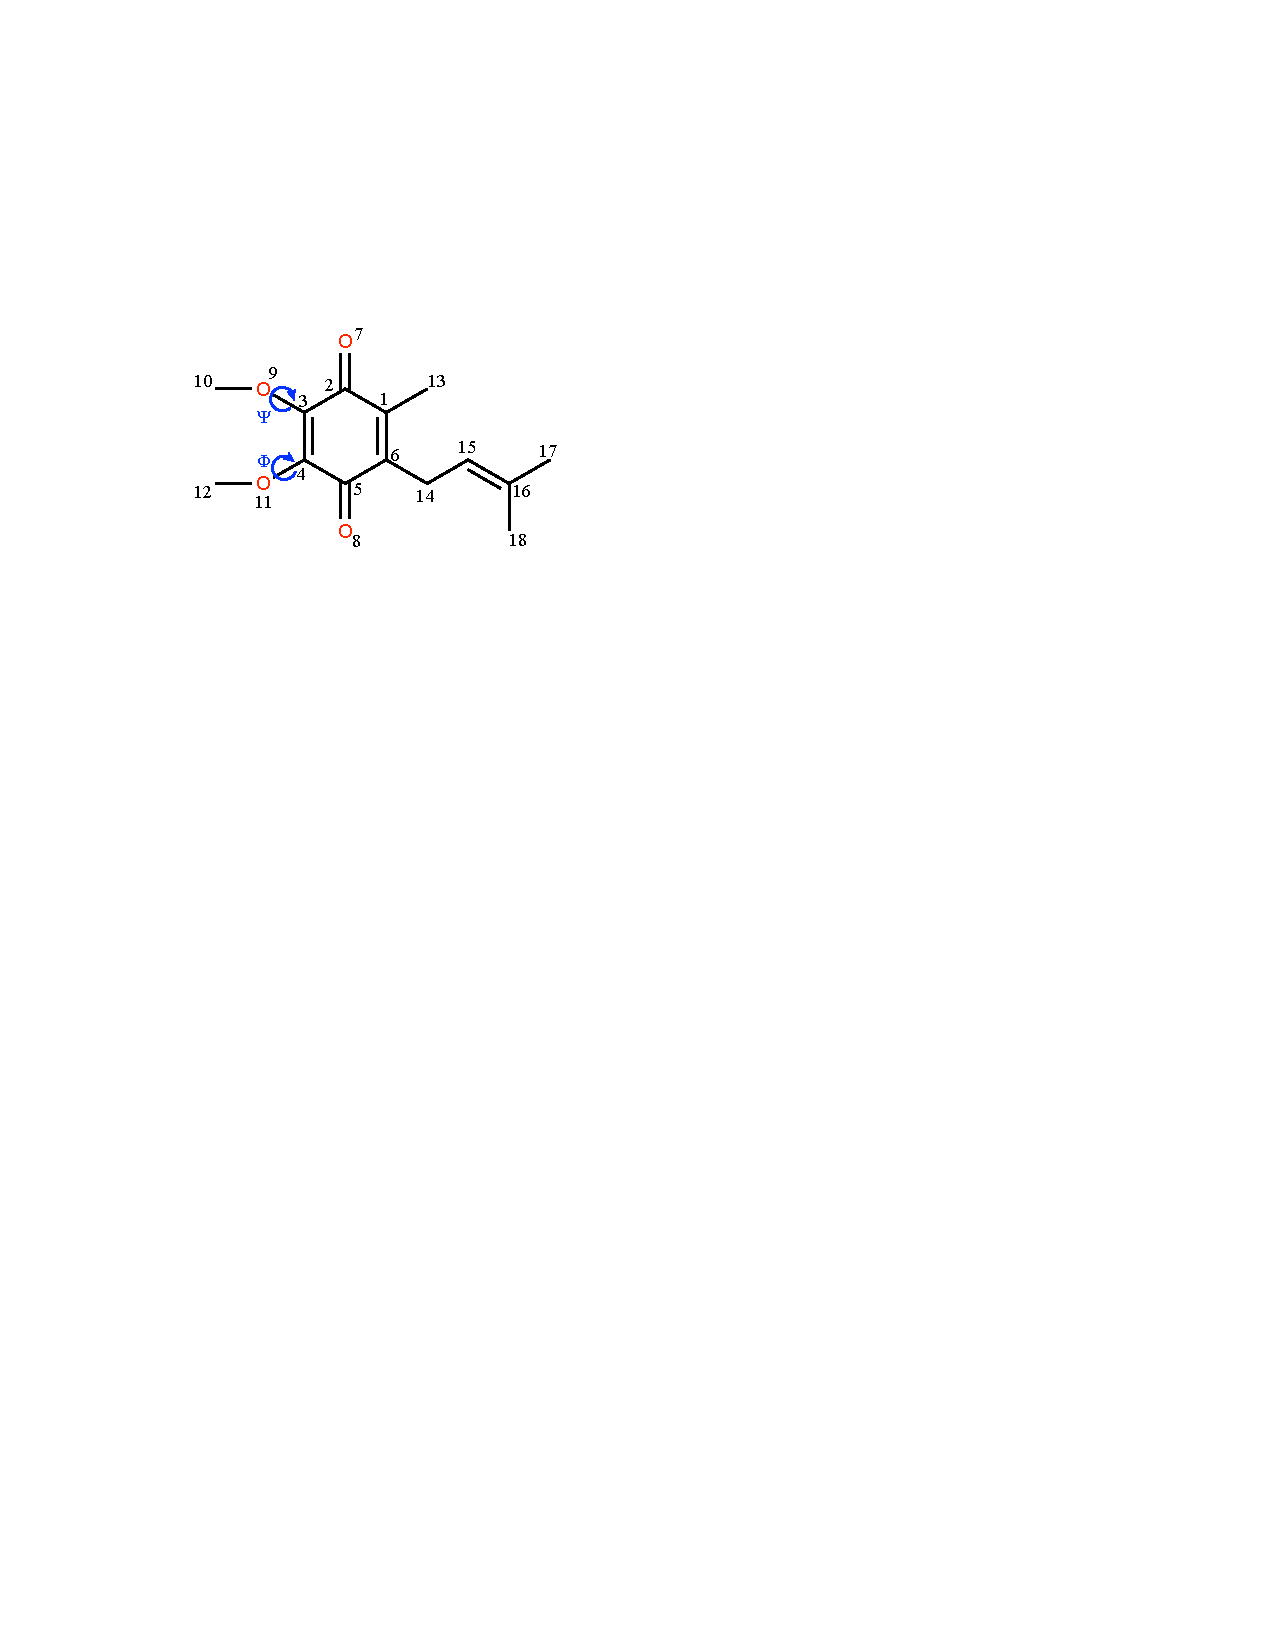
\includegraphics[width=0.5\textwidth]{chapters/methods/image/Q1-labelled.pdf}
    \caption{Skeletal diagram of Q\textsubscript{1}. Q\textsubscript{0} can be obtained by omitting the the isoprene tail (C atoms 14-18). The dihedral angles $\mathrm{\Psi}$ and $\mathrm{\Phi}$ are defined as the angle between the plane of the benzene ring and the plane of the methoxy groups.}\label{fig:quinone_dihedral_scan}
\end{figure}

The resultant structures served as the basis for subsequent EOM-EA-CC2 electron binding energy calculations. The RHF wavefunction for the neutral molecule was used as the reference for a subsequent CC2 calculation, which was then used to compute the EA-EOM-CC2 electron binding energy. An advantage of this method is that it provides the conformational energy of both the ground state and the anion states in one calculation. Unless otherwise specified, these calculations were performed with the aug-cc-pVDZ+6s3p basis set (\textit{vide supra}) to ensure an adequate description of non-valence states. In all cases, both the VBS and DBS are computed at once, as well as their corresponding Dyson orbitals. In all cases, spin scaling is omitted. %For the Dyson orbital computations, only right Dyson orbitals were calculated. This approach expedited the calculations by obviating the need to determine the lambda amplitudes.

%Hydrogens were added using \textit{PyMOL}'s \cite{PyMOL} \texttt{add\_H}  functionality, and relaxed using the method above (fixing the rest of the heavy atoms).\\

\subsection{Interaction Scans with Small Molecules}

Cluster models were constructed featuring second row hydrides (methane, ammonia, water and hydrogen fluoride) as a crude approximation to the solvent or functional group.
The models were based on the Q\textsubscript{0} structure with dihedral angles $\mathrm{\Psi=160}$\degree and $\mathrm{\Phi=-80}$\degree. The interacting molecule was positioned along the dipole moment vector of the quinone, originating from the Q\textsubscript{0} centre of the benzene ring. The dipole moments of the quinone and hydride were then aligned in either parallel or antiparallel orientations. The interaction distance was defined as the separation between the centre of benzene ring of the quinone and the heavy atom of the hydride.  The atoms of the quinone were frozen and interaction distance of the hydride was systematically varied along the dipole vector while keeping all its intramolecular coordinates fixed. These structures were not subjected to further optimisation and were used to compute the neutral total energy and the VBS and DBS electron binding energy using CC2 and EA-EOM-CC2/aug-cc-pVDZ+6s3p correspondingly. All geometries, along with the Python scripts used for their generation, are available in the \href{https://github.com/EliteSushi/TCCM_Thesis}{GitHub repository}.\\
%In the case of the noble gas cage, the centre of the benzene ring of Q\textsubscript{0} was coincident with the centre of the icosahedron.

%%%%%%%%%%%%%%%%%%%%%%%%%%%%%%%%%%%%%%%%%%%%%%%%%%
% Keep the following \cleardoublepage at the end of this file,
% otherwise \includeonly includes empty pages.
\cleardoublepage

% vim: tw=70 nocindent expandtab foldmethod=marker foldmarker={{{}{,}{}}}